% 导言区
\documentclass[12pt]{article} % book report  letter
\usepackage{ctex}  % 使用中文包
\usepackage{graphicx}
\usepackage{amsmath}
\usepackage{amssymb}
\graphicspath{{figures/}, {figures/result}} %图片在当前目录下的figures目录
\bibliographystyle{plain}% plain  unsrt  alpha  abbrv

\newcommand\degree{^\circ}
\newcommand{\myfont}{\textit{\textbf{\textsf{Fancy Text}}}}

\title{\songti 勾股定理}
\author{\heiti 周方全}
\date{\today}


% 正文区

\begin{document}
	\maketitle
	\section{一些格式设置}
	Hello World!
	
	$f(x)$
	
	\subsection {字体的设置}
	\textrm{Roman Family} 
	\textsf{Sans Serif Family}
	\texttt{Typewriter Family}
	
	{\rmfamily Roman Family} 
	{\sffamily Sans Serif Eamily} 
	{\ttfamily Typewriter Family}
	
	{\sffamily who you are? you find self on everyone around. take you as the same as others !}
	
	{\ttfamily Are you wiser than others? definitely no. in some ways,may it is true. What can you achieve? a luxurious house? abrillilant car? an admirable career? who knows?}
	
	\subsection {字体系列设置(粗细、宽度)}
	\textmd{Medium Series} 
	\textbf{Boldface Series}
	
	{\mdseries Medium series} 
	{\bfseries Boldface Series}
	
	\subsection {字体形状(直立、斜体、伪斜体、小型大写)}
	\textup{Upright Shape} 
	\textit{Italic Shape}
	\textsl{S1anted Shape} 
	\textsc{Small caps Shape}
	
	{\upshape Upright Shape} 
	{\itshape Italic Shape} 
	{\slshape Slanted Shape} 
	{\scshape Small caps Shape}
	
	\subsection {中文字体}
	{\songti\it 宋体} \quad 
	{\heiti 黑体}  \quad 
	{\fangsong 仿宋}\quad 
	{\kaishu 楷书}
	
	中文字体的 \textbf{粗体}与 \textit{斜体}
	
	\subsection {字体大小}
	{\tiny	       Hello}\\
	{\scriptsize   Hello}\\
	{\footnotesize Hello}\\
	{\small        Hello}\\
	{\normalsize   Hello}\\
	{\large        Hello}\\
	{\Large        Hello}\\
	{\LARGE        Hello}\\
	{\huge         Hello}\\
	{\Huge         Hello}
	
	\subsection{中文字号设置命令}
	\zihao{3} 你好!
	
	{\myfont 你好!}
	
	\section{图片}
	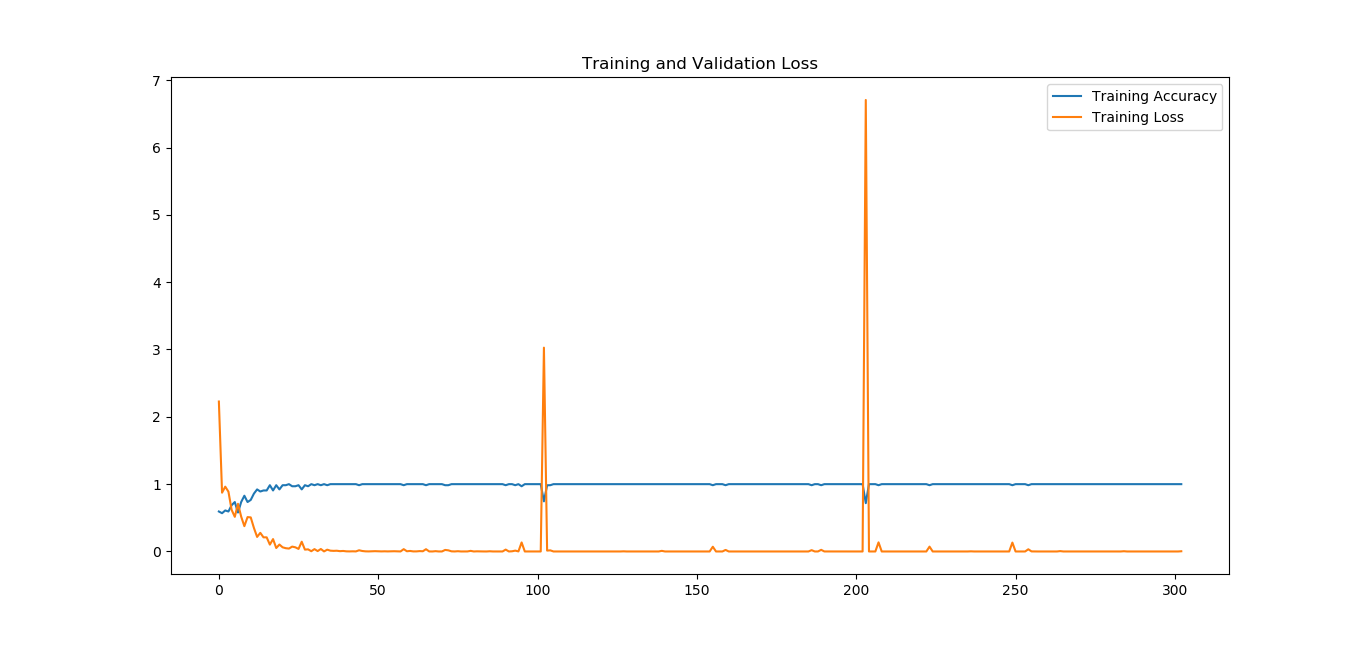
\includegraphics{CNN.png}
	
	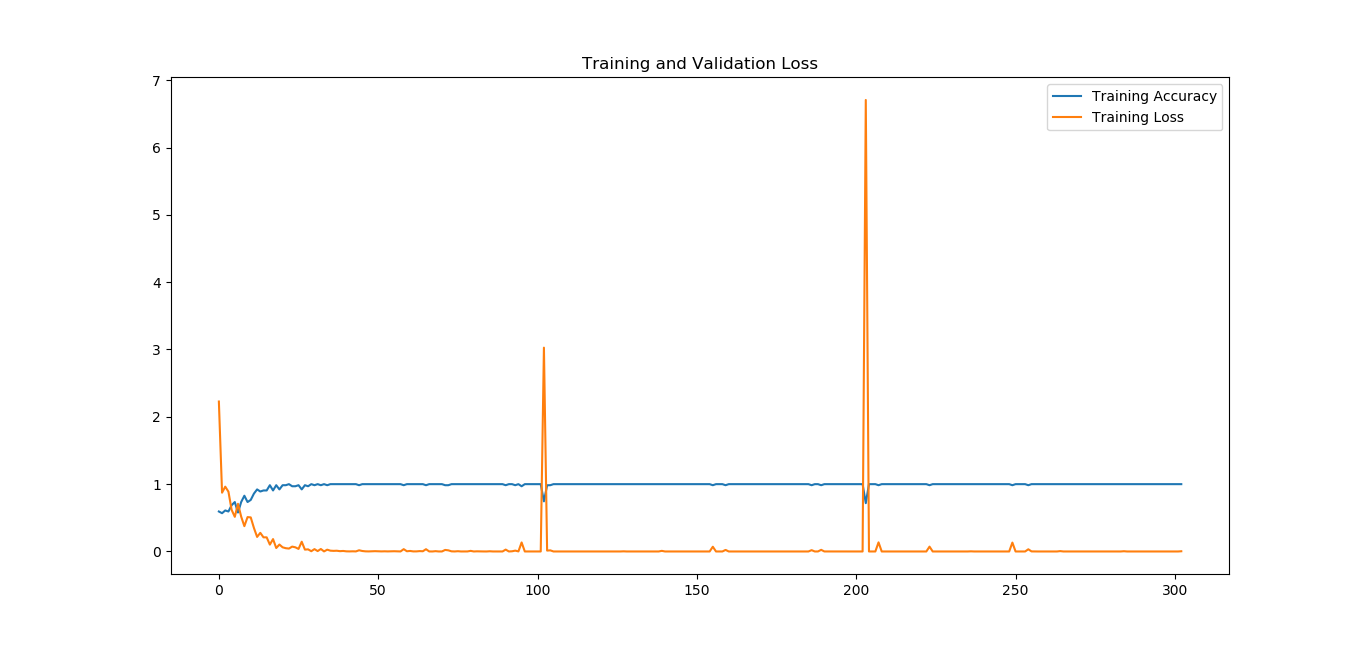
\includegraphics[scale=0.3]{CNN}
	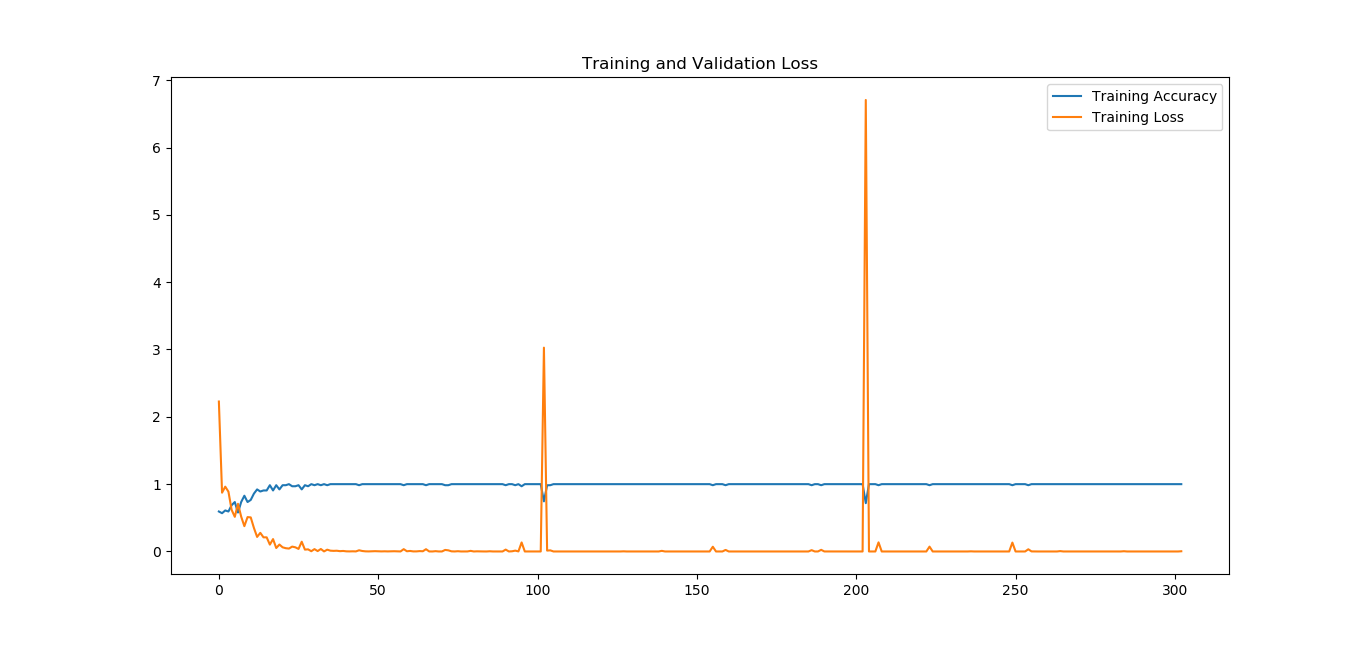
\includegraphics[scale=0.03]{CNN}
	
	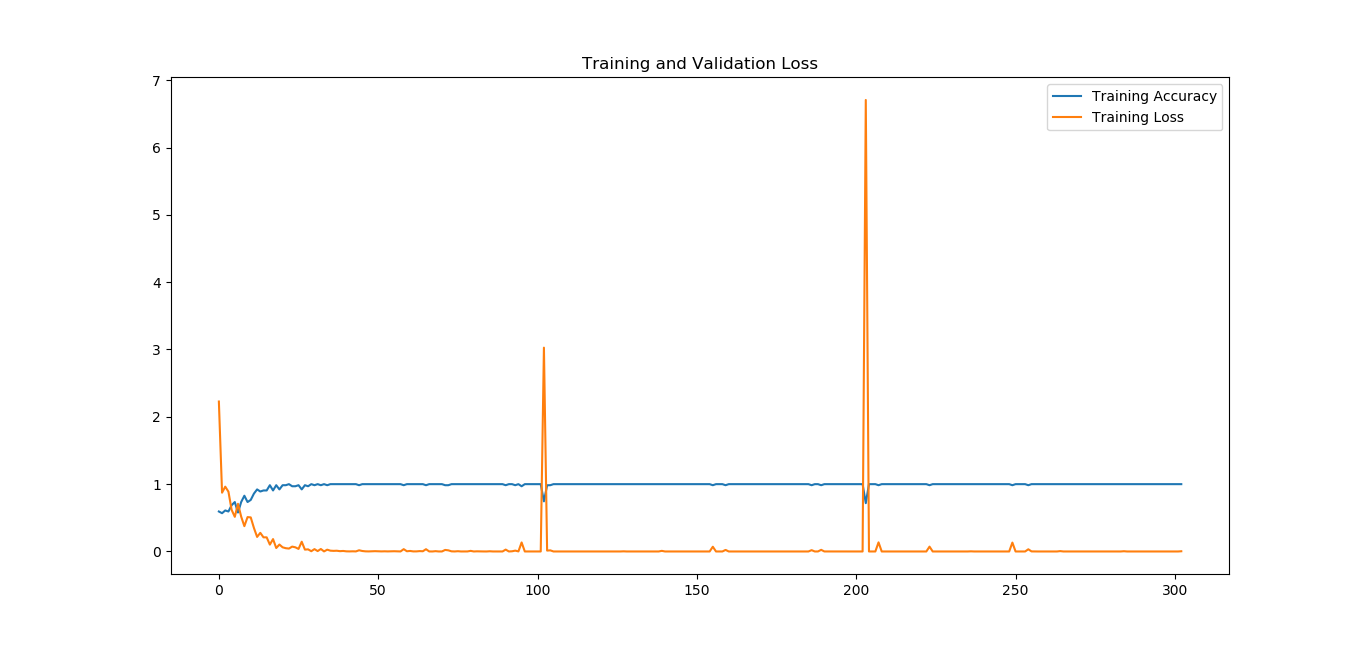
\includegraphics[height=2cm]{CNN}
	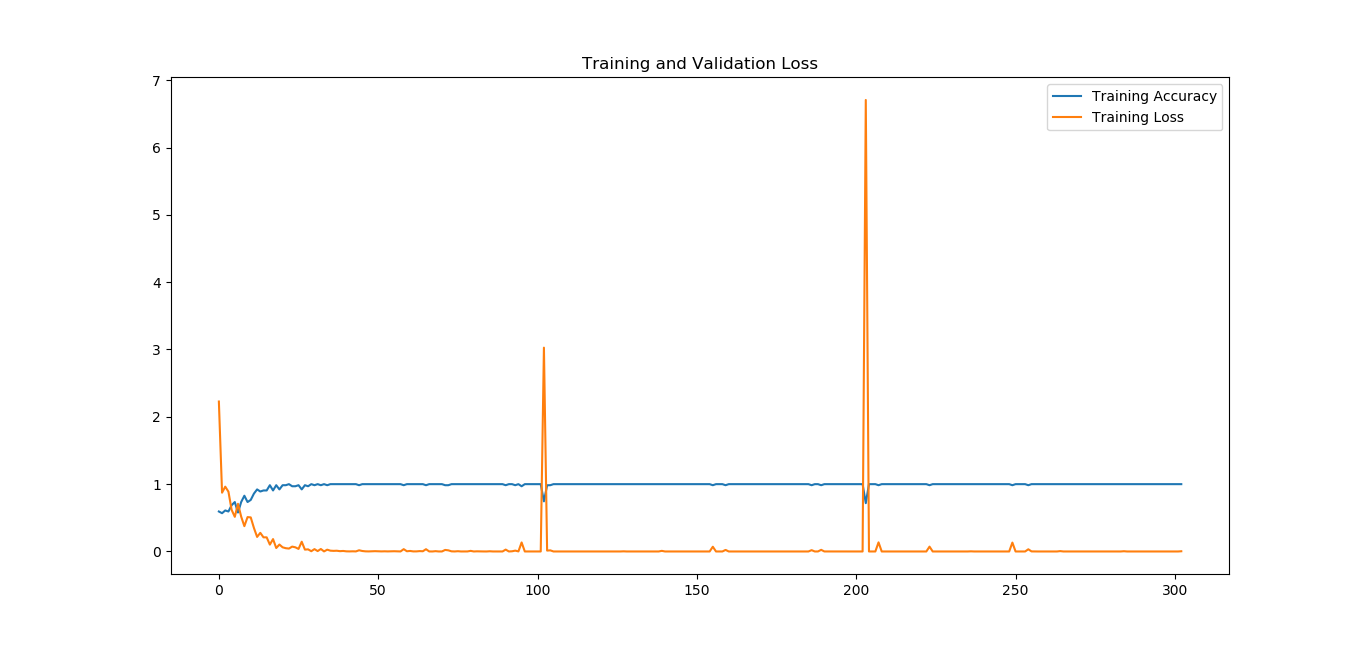
\includegraphics[height=4cm]{CNN}
	
	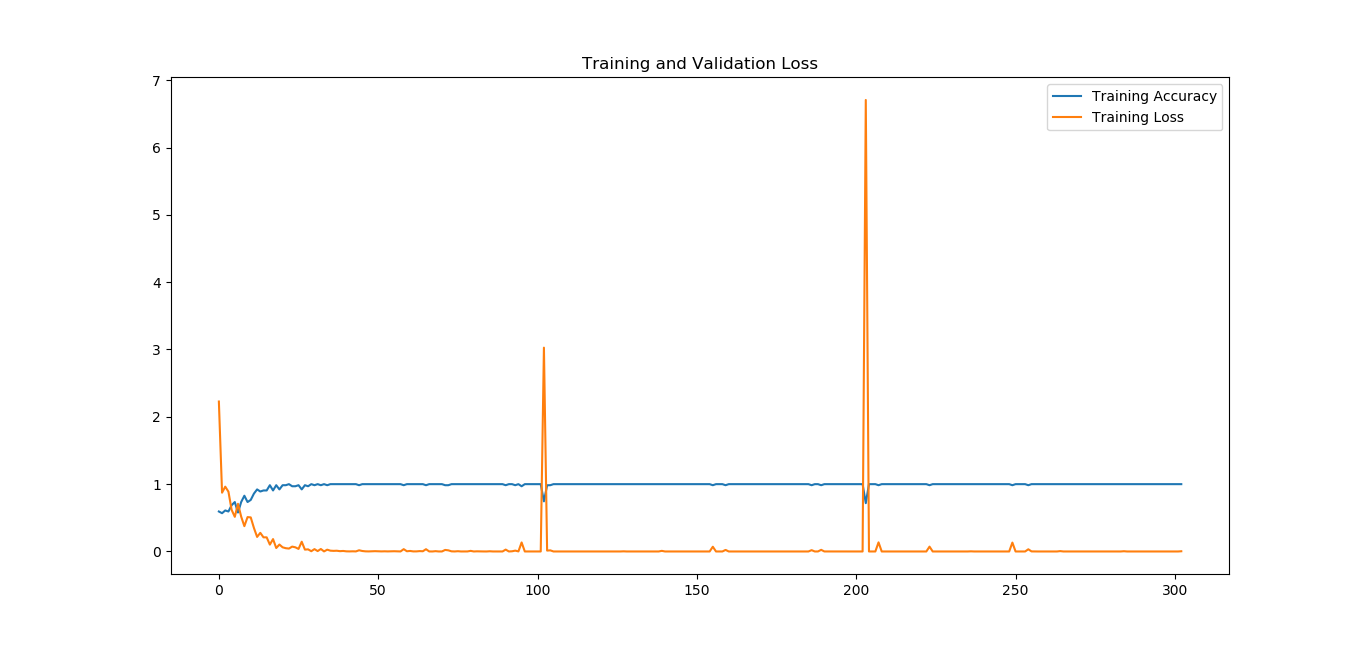
\includegraphics[width=2cm]{CNN}
	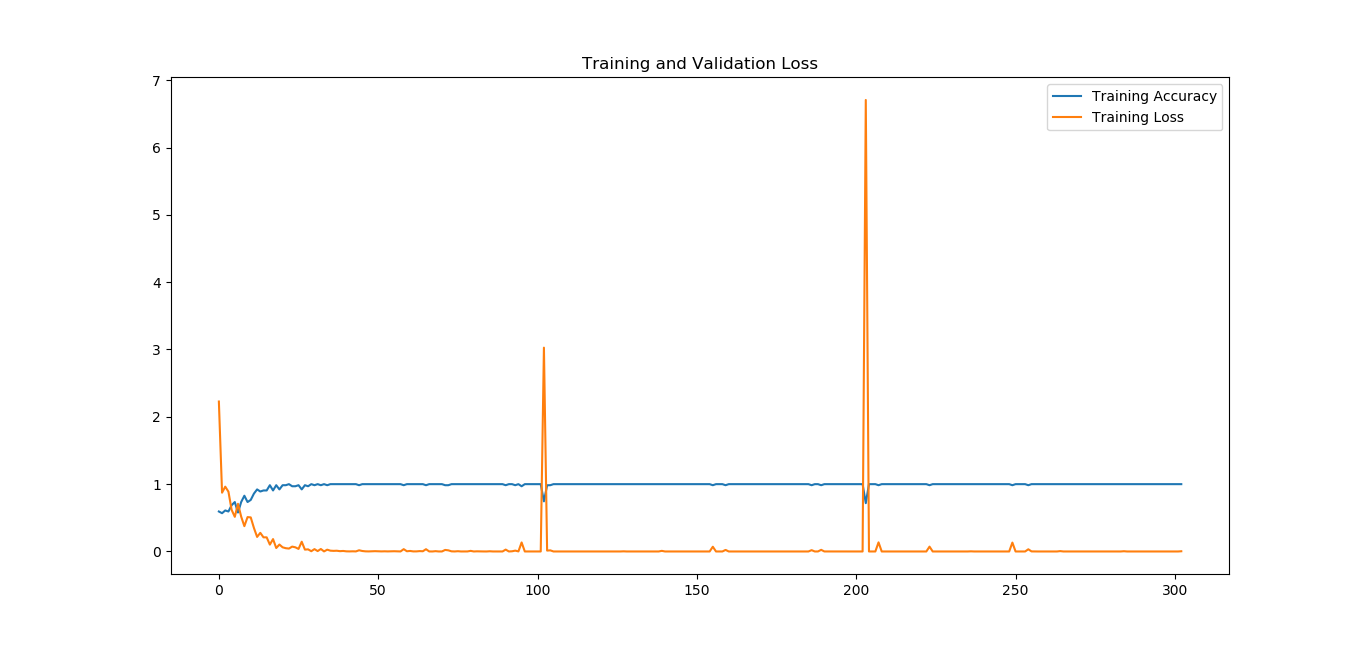
\includegraphics[width=4cm]{CNN}
	
	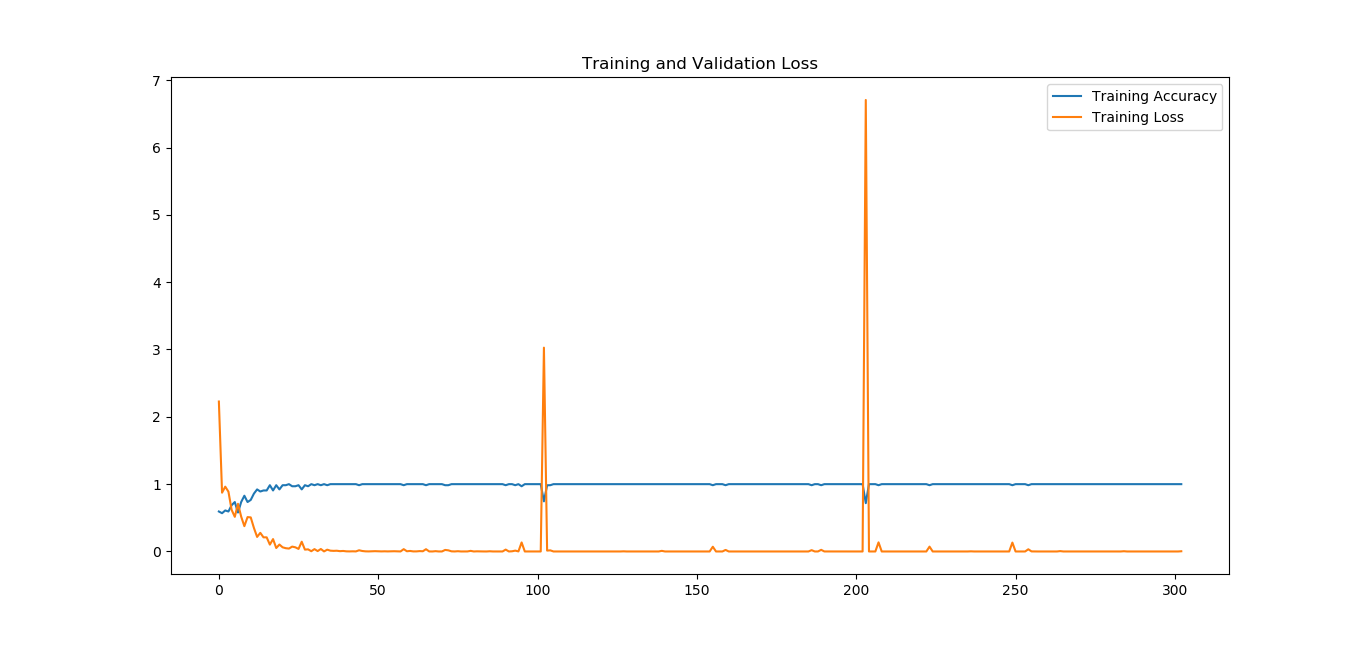
\includegraphics[height=0.1\textheight]{CNN}
	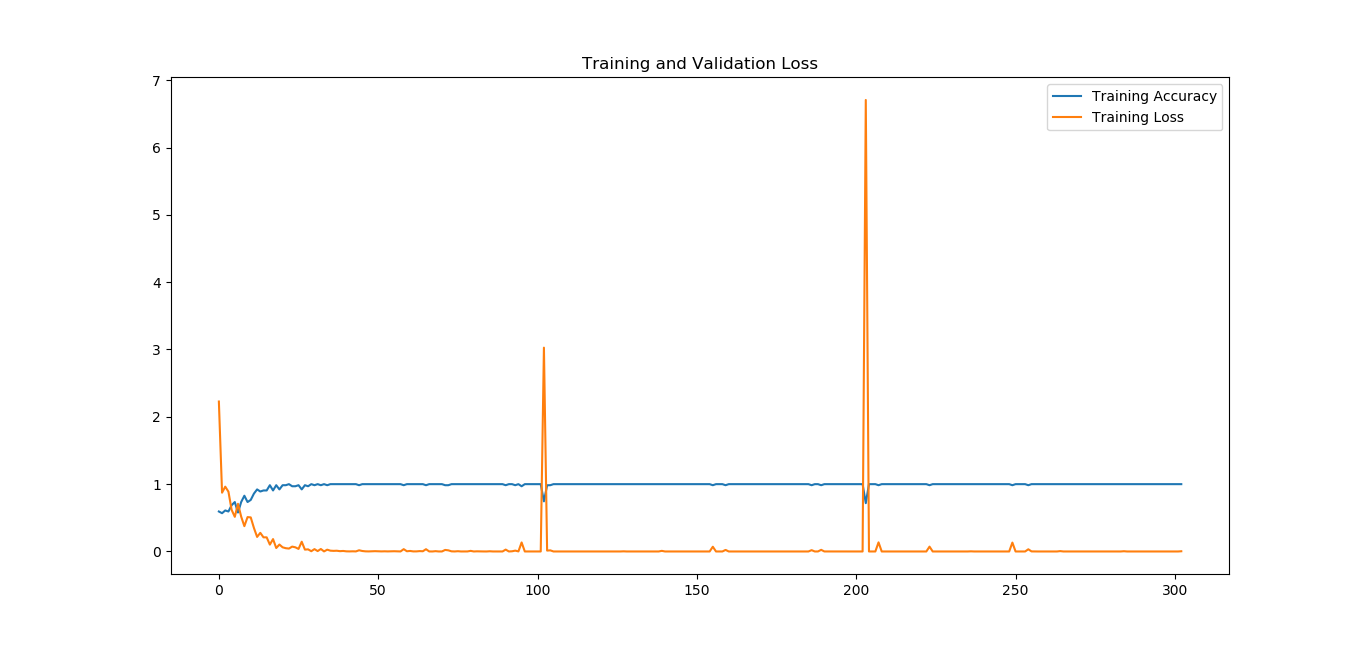
\includegraphics[height=0.3\textheight]{CNN}
	
	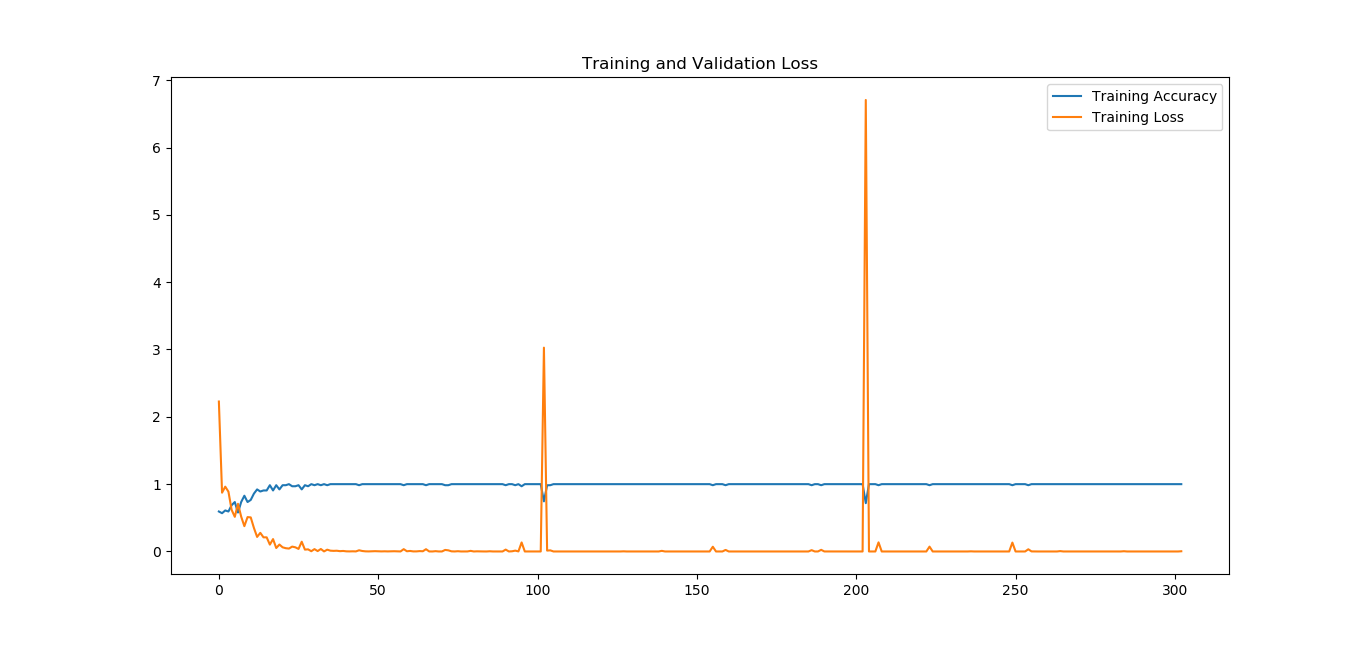
\includegraphics[width=0.1\textwidth]{CNN}
	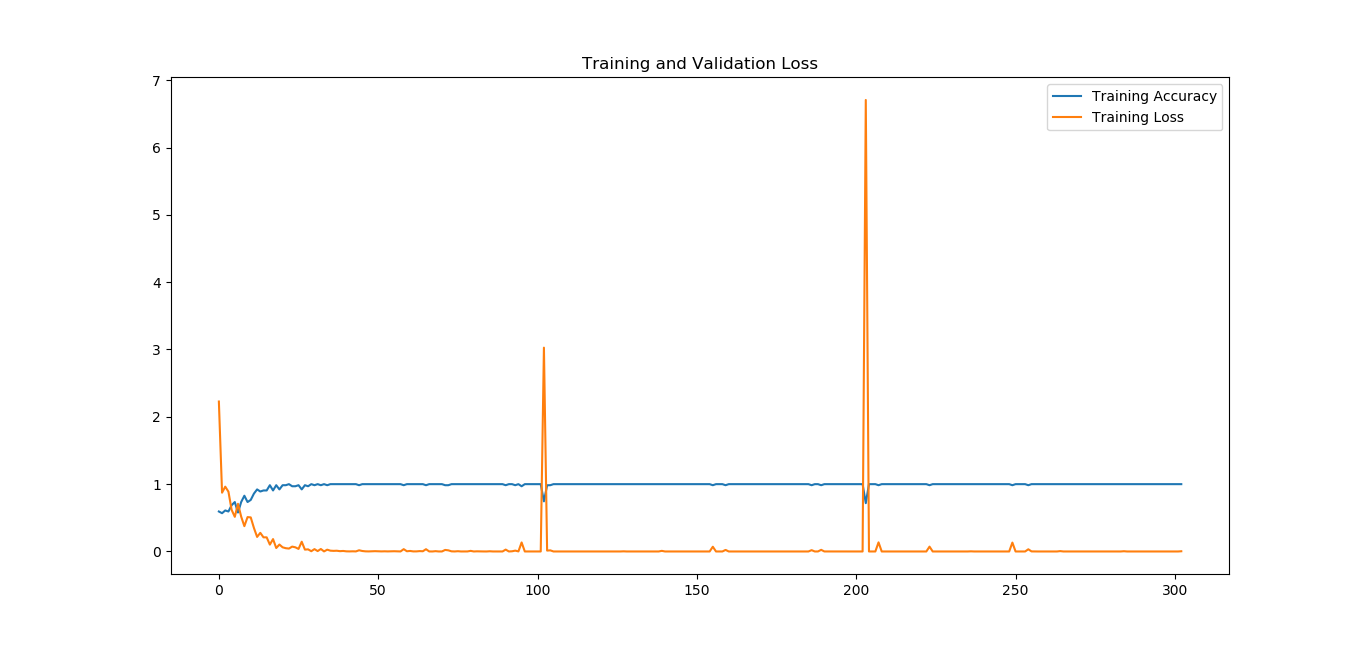
\includegraphics[width=0.2\textwidth]{CNN}
	
	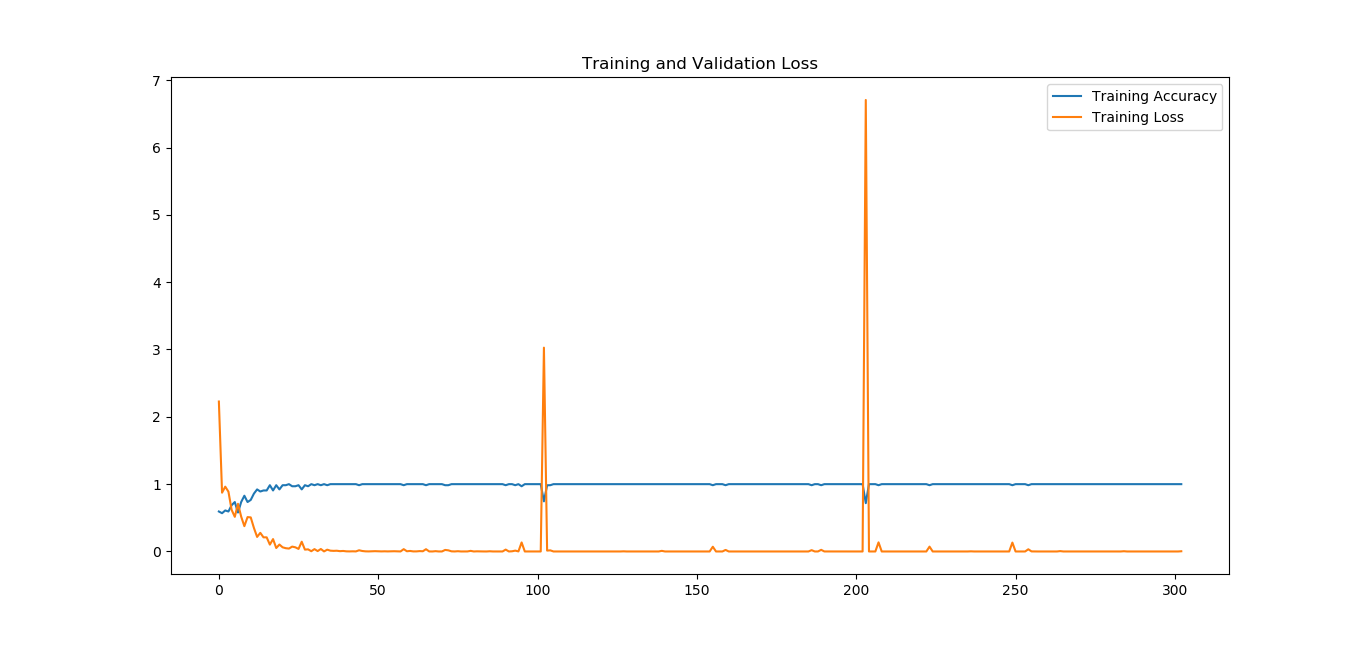
\includegraphics[angle=45, height=0.2\textheight]{CNN}
	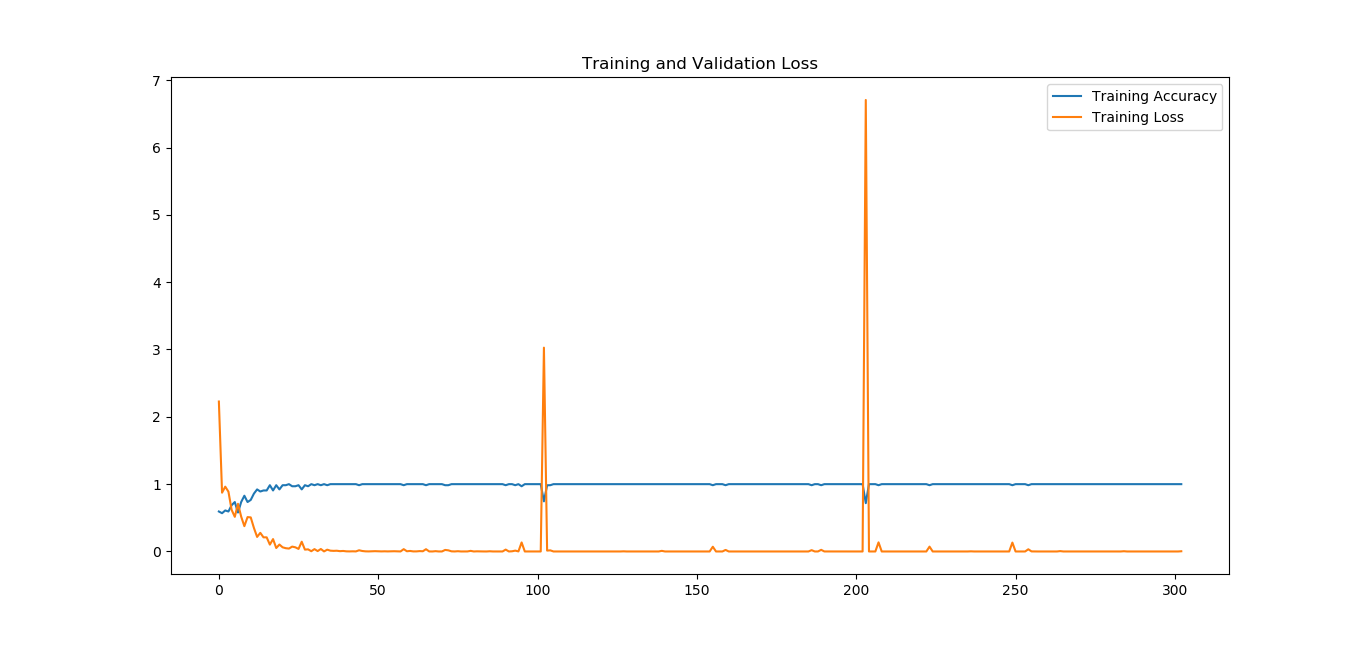
\includegraphics[angle=90, width=0.2\textwidth]{CNN}
	
	\section{表格}
	
	\begin{tabular}{l c c c r}
		\hline
		训练轮次 & 损失值 & 准确率 & 耗时/秒 \\
		\hline
		1 & 0.8542 & 0.501 & 118.4  \\
		2 & 0.6492 & 0.6622 & 122.5 \\
		3 & 0.3288 & 0.8411 & 116.2 \\
		4 & 0.2542 & 0.8822 & 106.1 \\
		\hline
	\end{tabular}


	\begin{tabular}{|l|c|c|c|r}
		\hline
		训练轮次 & 损失值 & 准确率 & 耗时/秒 \\
		\hline
		1 & 0.8542 & 0.501 & 118.4  \\
		2 & 0.6492 & 0.6622 & 122.5 \\
		3 & 0.3288 & 0.8411 & 116.2 \\
		4 & 0.2542 & 0.8822 & 106.1 \\
		\hline
	\end{tabular}


	\begin{tabular}{|l||c|c|c|r}
		\hline
		训练轮次 & 损失值 & 准确率 & 耗时/秒 \\
		\hline\hline
		1 & 0.8542 & 0.501 & 118.4  \\
		2 & 0.6492 & 0.6622 & 122.5 \\
		3 & 0.3288 & 0.8411 & 116.2 \\
		4 & 0.2542 & 0.8822 & 106.1 \\
		\hline
	\end{tabular}
	
	更多工具在命令窗口输入:texdoc longtab、texdoc tabu
	
	\subsection{浮动体}
	
	如图\ref{fig-CNN},是卷积神经网络的一个简单地模型。
	\begin{figure}[htbp]
		\centering
		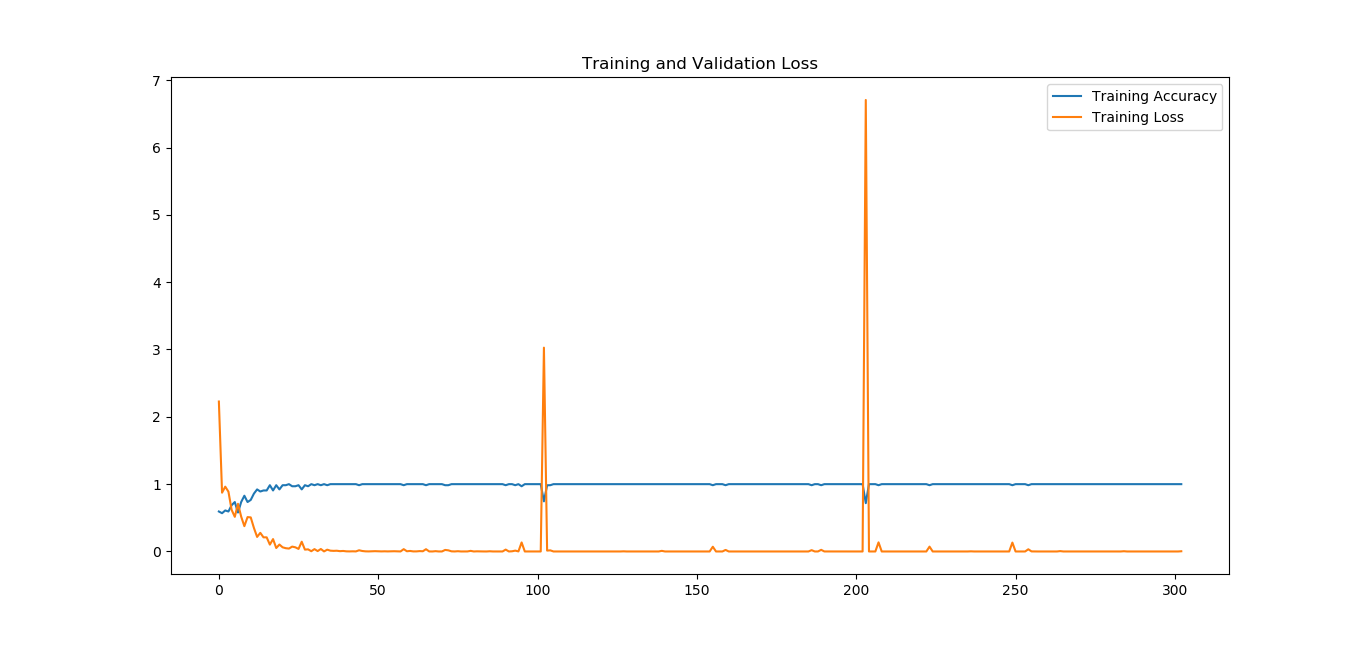
\includegraphics[height=0.3\textheight]{CNN}
		\caption{CNN结果模型图}
		\label{fig-CNN}     % 个图形写一个标签。
	\end{figure}
	
	如表\ref{tab-result},是卷积神经网络的一个简单地模型。
	\begin{table}
		\centering
		\caption{训练结果}
		\label{tab-result}
		\begin{tabular}{|l||c|c|c|r}
			\hline
			训练轮次 & 损失值 & 准确率 & 耗时/秒 \\
			\hline\hline
			1 & 0.8542 & 0.501 & 118.4  \\
			2 & 0.6492 & 0.6622 & 122.5 \\
			3 & 0.3288 & 0.8411 & 116.2 \\
			4 & 0.2542 & 0.8822 & 106.1 \\
			\hline
		\end{tabular}
	\end{table}
	
	\section{矩阵排版}
	\section{多行公式排版}
	
	\begin{gather}
		a + b = c \\ 
		c = a + b
	\end{gather}
	
	\begin{gather*}
		a + b = c \\ 
		c = a \times b
	\end{gather*}

	\begin{gather}
		a + b = c \notag \\ 
		c = a + b
	\end{gather}
		
	\begin{align}  % 该环境可以用&对其
		a + b &= c \\ 
		c &= a + b \notag
	\end{align}

	\begin{align*}  % 该环境可以用&对其
		a + b &= c \\ 
		c &= a + b
	\end{align*}

	\begin{equation}
		\begin{split}
			lcos 2x &= \cos^2 x - lsin^2 x \\ 
			&= 2\cos^2 x - 1
		\end{split}
	\end{equation}

	\begin{equation}
	D(x) = \begin{cases}
		1, &\text{如果 } x \in \mathbb{Q}; \\ 
		0, &\text{如果 } x \in \mathbb{R}\setminus\mathbb{Q}
	\end{cases}
	\end{equation}
	
	
	
	
	\section{自然语言处理相关知识}
		\subsection{词频-逆向文件频率}
		\subsection{文本预处理}
		\subsection{连续词袋模型}
	\section{深度学习相关知识}
		\subsection{激活函数}
		\subsection{反向传播算法}
		\subsection{卷积神经网络}
		\subsection{循环神经网络}
			\subsubsection{长短期记忆网络}
		\subsection{Transformer模型}
	\section{实验部分}
		\subsection{LSTM+Attention模型实验设计}
		\subsection{Transformer模型实验设计}
	\section{结果与展望}
		\subsection{总结}
		\subsection{不足之处及未来展望}
	
	
	\section{一些格式设置}
	\maketitle
	Hello World!
	
	$f(x)$
	
	% 字体的设置
	\textrm{Roman Family} \textsf{Sans Serif Family}
	\texttt{Typewriter Family}
	
	{\rmfamily Roman Family} {\sffamily Sans Serif Eamily} 
	{\ttfamily Typewriter Family}
	
	{\sffamily who you are? you find self on everyone around. take you as the same as others !}
	
	{\ttfamily Are you wiser than others? definitely no. in some ways,may it is true. What can you achieve? a luxurious house? abrillilant car? an admirable career? who knows?}
	
	%字体系列设置(粗细、宽度)
	\textmd{Medium Series} \textbf{Boldface Series}
		
	{\mdseries Medium series} {\bfseries Boldface Series}
	
	%字体形状(直立、斜体、伪斜体、小型大写)
	\textup{Upright Shape} 
	\textit{Italic Shape}
	\textsl{S1anted Shape} 
	\textsc{Small caps Shape}
	
	{\upshape Upright Shape} 
	{\itshape Italic Shape} 
	{\slshape Slanted Shape} 
	{\scshape Small caps Shape}
	
	%中文字体
	{\songti\it 宋体} \quad 
	{\heiti 黑体}  \quad 
	{\fangsong 仿宋}\quad 
	{\kaishu 楷书}
	
	中文字体的 \textbf{粗体}与 \textit{斜体}
	
	%字体大小
	{\tiny	       Hello}\\
	{\scriptsize   Hello}\\
	{\footnotesize Hello}\\
	{\small        Hello}\\
	{\normalsize   Hello}\\
	{\large        Hello}\\
	{\Large        Hello}\\
	{\LARGE        Hello}\\
	{\huge         Hello}\\
	{\Huge         Hello}

	% 中文字号设置命令
	\zihao{3} 你好!
	
	{\myfont 你好!}
	
	
	\section{参考文献}
	\subsection{BibTex}
	这是一个参考文献的引用: \cite{1}
	这是另一个引用: \cite{付盼盼2021疫情背景下线上教学在计算机辅助产品设计中的应用研究}
		
%	\begin{thebibliography}{99}	
%\bibitem{article1}陈立辉,苏伟,蔡川,陈晓云.\emph{基于LaTex的web数学公式提取方法研究}[7].计算机科学.2014(06)
%	\end{thebibliography}
	
	
	
	%这是一个参考文献的引用: \cite{mittelbach2004}
	%这是另一个引用: \cite{patashnik1988designing}
	\bibliography{reference}
	
		\subsection{BibLaTex}
	
	
	
\end{document}